\subsection{UC3 - Ordinazione collaborativa}\label{usecase:3}

\begin{figure}[H]
    \centering
    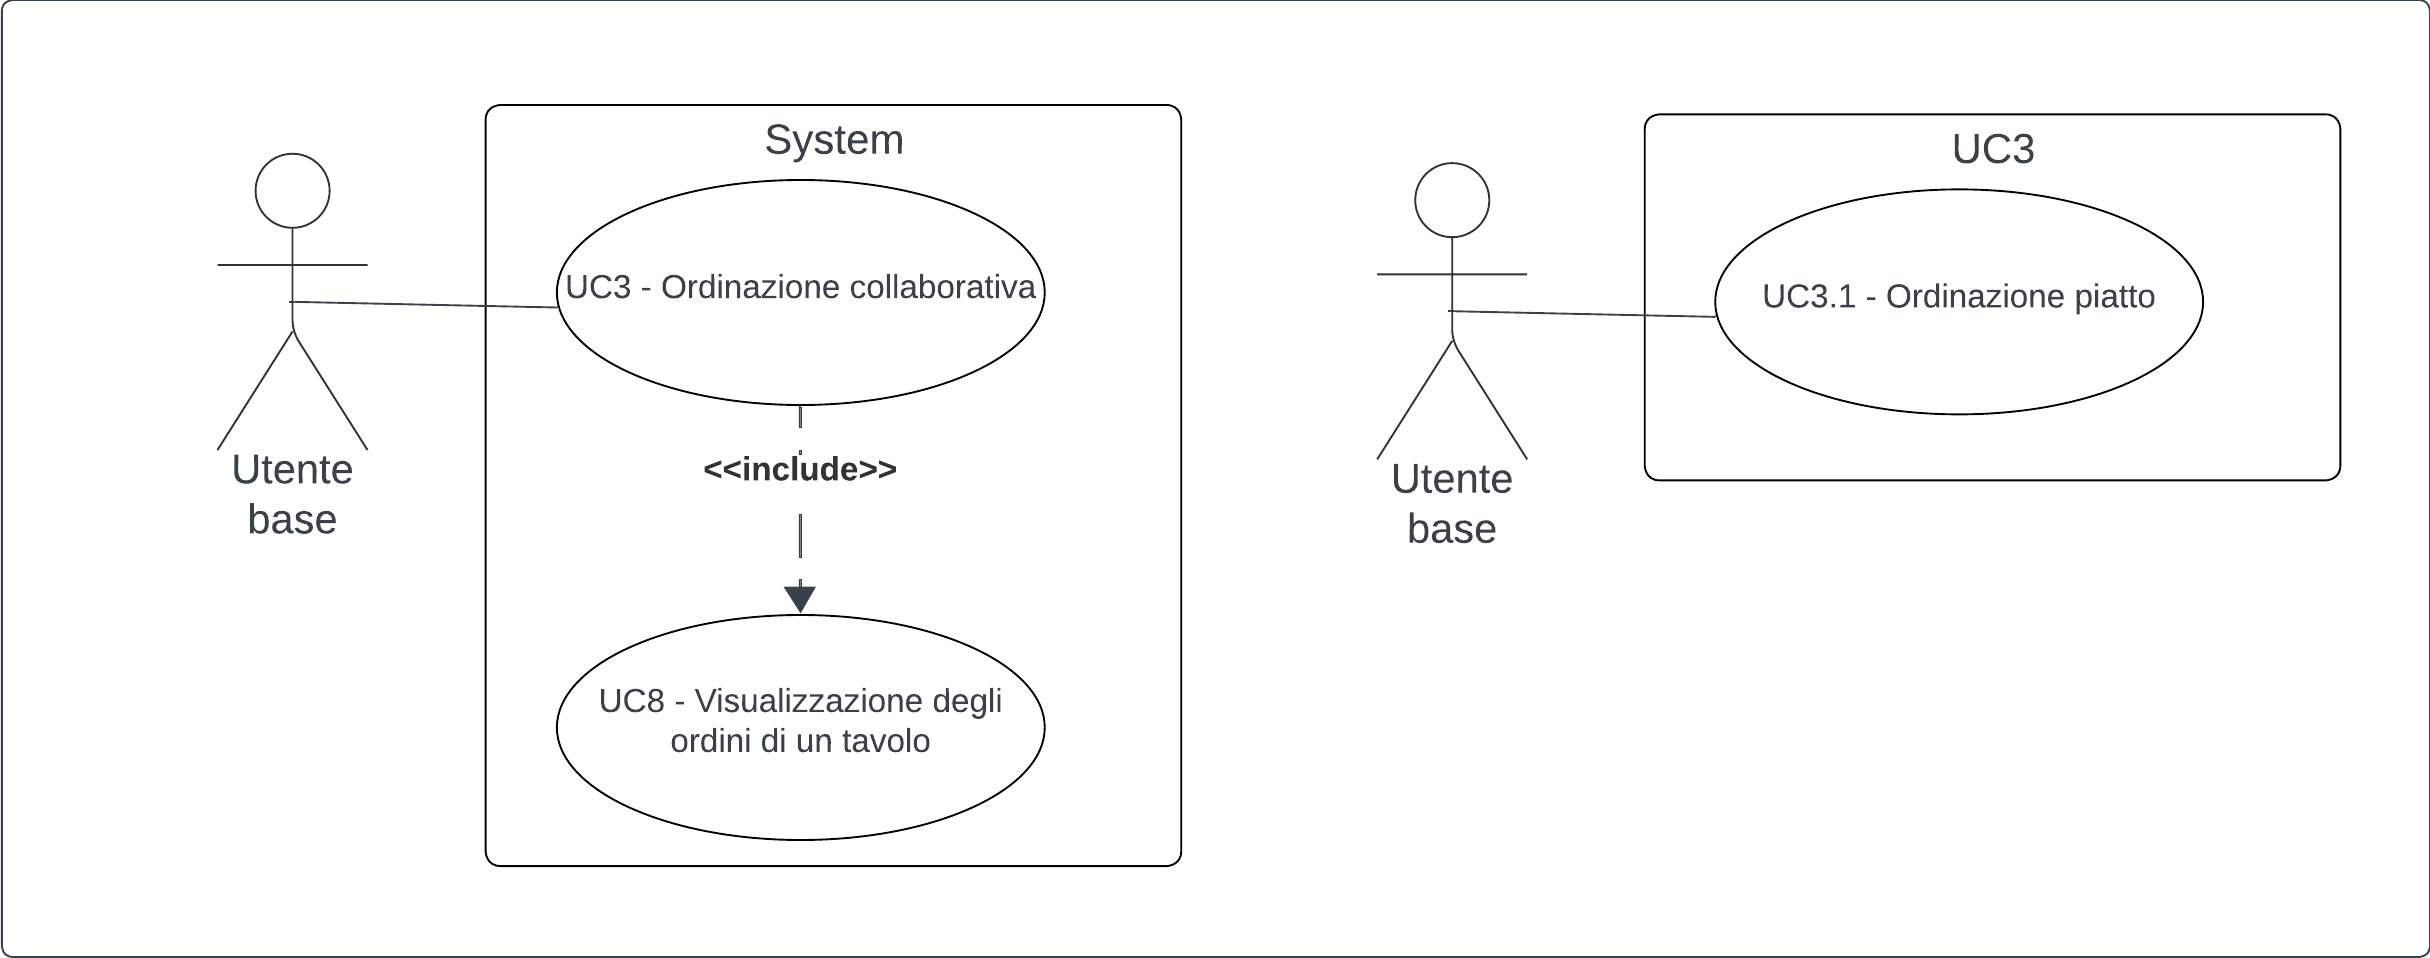
\includegraphics[width=0.9\linewidth]{ucd/UCD3_nuovo.png}
\end{figure}

\textbf{Attori}:
\begin{itemize}
    \item Utente base
\end{itemize}
\textbf{Precondizioni}:
\begin{itemize}
    \item L'utente è autenticato dal $\textit{Sistema}_G$ 
    \item L'utente ha prenotato un tavolo (\nameref{usecase:23})
    \item La $\textit{Prenotazione}_G$ associata all'ordinazione è stata accettata dall'utente amministratore del ristorante (\nameref{usecase:19})
    \item Il limite di tempo per l'ordinazione non è ancora scaduto
\end{itemize}
\textbf{Postcondizioni}:
\begin{itemize}
    \item L'utente ha confermato la propria ordinazione delle pietanze associata ad una prenotazione.
\end{itemize}
\textbf{Scenario principale}:
\begin{enumerate}
    \item L'utente crea il proprio ordine:
    \begin{itemize}
    \item L'utente sceglie il pasto da ordinare (\nameref{usecase:3_1}); nel caso in cui la pietanza ordinata contenga allergeni segnalati dall'utente in fase di registrazione, deve essere notificato prima di  aggiungere la pietanza all'ordine.
    \item L'utente può scegliere di: modificare la quantità degli ingredienti; rimuoverne alcuni ingredienti; aggiungere degli ingredienti (\nameref{usecase:3_1}).
    \end{itemize}
    \item L'utente visualizza il riepilogo del suo ordine e quelli degli altri utenti con cui ha prenotato il tavolo (\nameref{usecase:8}).
    \item L'utente conferma l'ordinazione.
    \item Il $\textit{Sistema}_G$ notifica il ristorante mediante \textit{push-notification}.
\end{enumerate}


\subsubsection{UC3.1 - Ordinazione piatto}\label{usecase:3_1}

\textbf{Attori}:
\begin{itemize}
    \item Utente base autenticato
\end{itemize}
\textbf{Precondizioni}:
\begin{itemize}
    \item L'utente è autenticato dal $\textit{Sistema}_G$ 
    \item L'utente ha prenotato un tavolo (\nameref{usecase:23})
    \item La $\textit{Prenotazione}_G$ associata all'ordinazione è stata accettata dall'utente amministratore del ristorante (\nameref{usecase:19})
    \item Il limite di tempo per l'ordinazione non è ancora scaduto
\end{itemize}
\textbf{Postcondizioni}:
\begin{itemize}
    \item L'utente ha ordinato il piatto
\end{itemize}
\textbf{Trigger}:
\begin{itemize}
    \item L'utente vuole aggiungere un piatto alla ordinazione collaborativa
\end{itemize}
\textbf{Scenario principale}:
\begin{enumerate}
    \item L'utente sceglie tra la lista delle pietanze una che vuole aggiungere al proprio ordine
    \item L'utente sceglie la quantità della pietanza
    \item Di ogni pietanza:
    \begin{itemize}
        \item L'utente visualizza gli ingredienti
        \item L'utente può aggiungere ingredienti
        \item L'utente può rimuovere ingredienti
    \end{itemize}
    \item L'utente conferma il piatto
\end{enumerate}
\newpage

\begin{comment}
\subsection{UC3 - Ordinazione collaborativa}\label{usecase:3}

\begin{figure}[H]
    \centering
    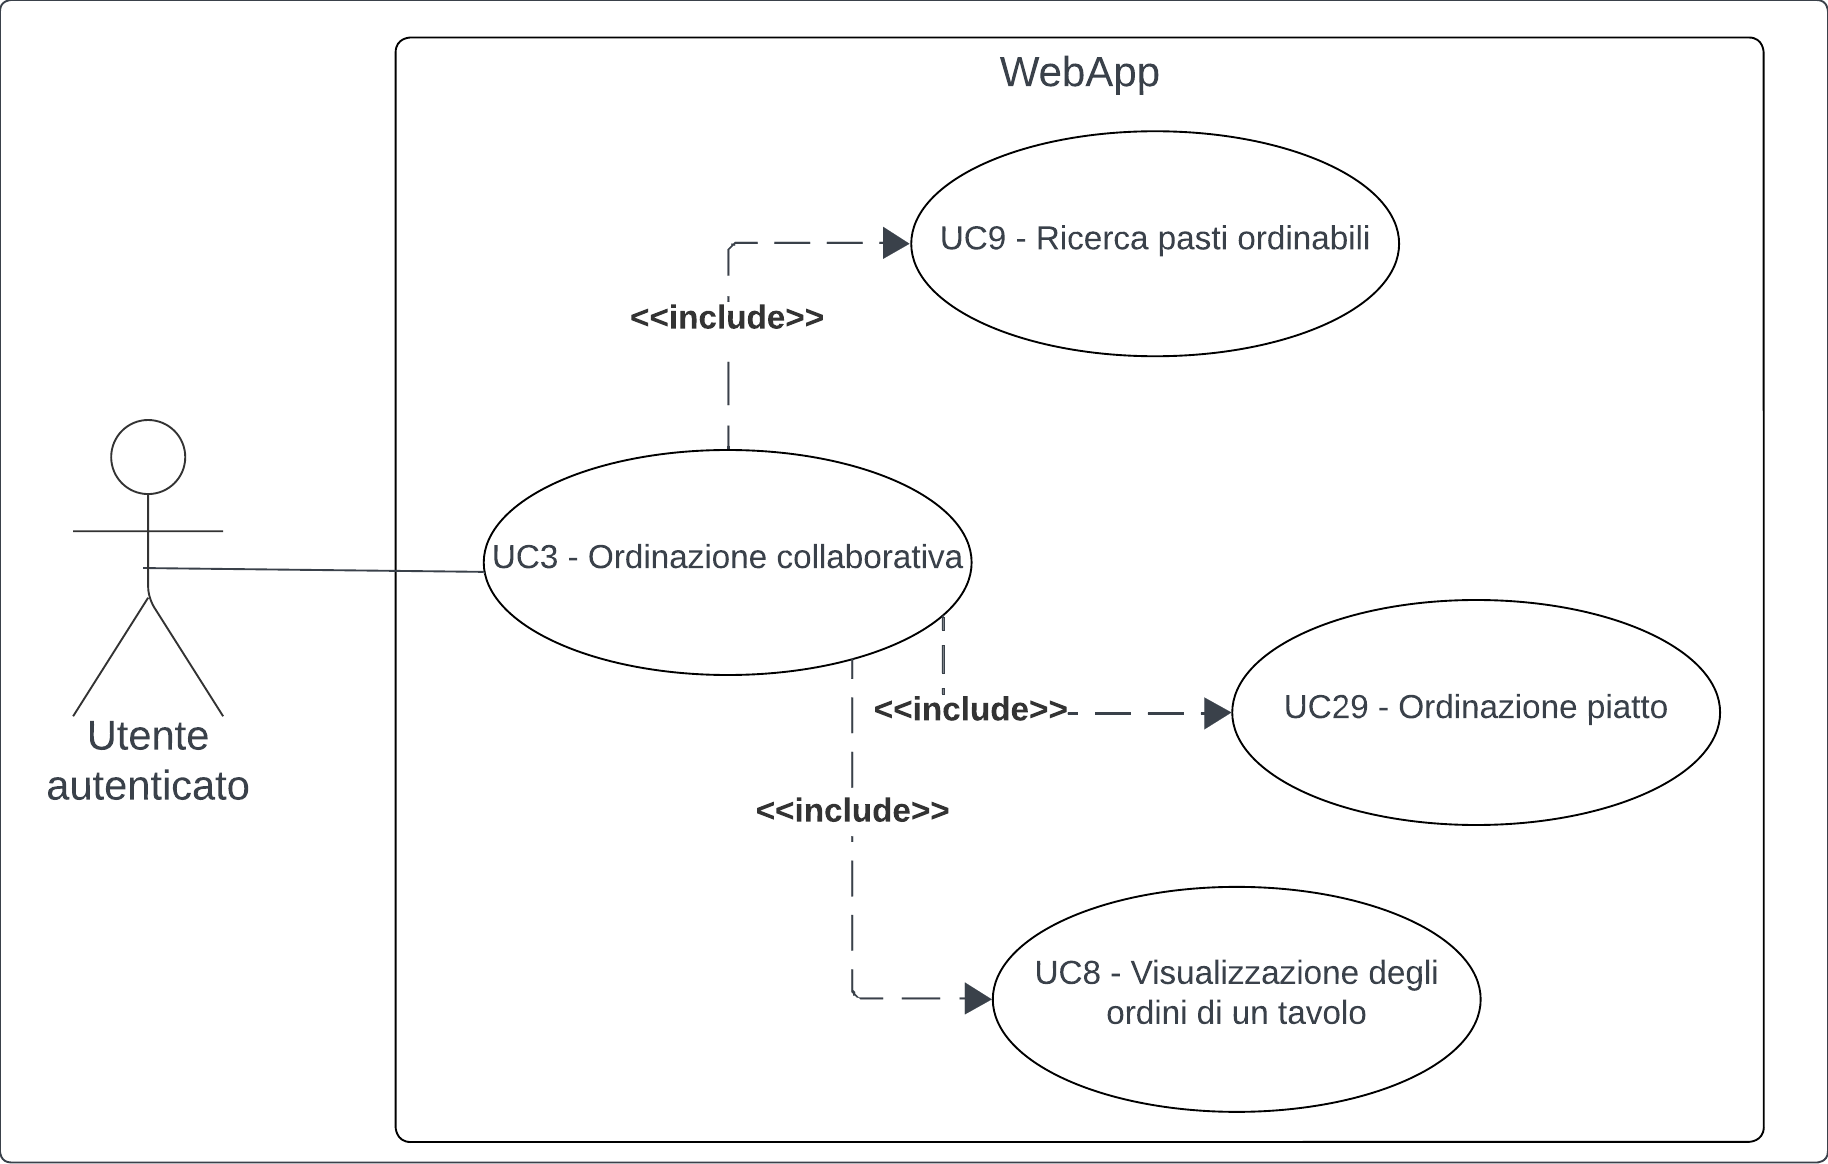
\includegraphics[width=0.9\linewidth]{ucd/UCD3.png}
\end{figure}

\textbf{Attori}:
\begin{itemize}
    \item Utente base autenticato
\end{itemize}
\textbf{Precondizioni}:
\begin{itemize}
    \item L'utente è autenticato dal $\textit{Sistema}_G$ 
    \item L'utente ha prenotato un tavolo (\nameref{usecase:23})
    \item La $\textit{Prenotazione}_G$ associata all'ordinazione è stata accettata dall'utente amministratore del ristorante (\nameref{usecase:19})
    \item Il tempo per l'ordinazione non è scaduto
\end{itemize}
\textbf{Postcondizioni}:
\begin{itemize}
    \item L'utente ha confermato l'ordinazione delle pietanze associata ad una prenotazione.
\end{itemize}
\textbf{Scenario principale}:
\begin{enumerate}
    \item L'utente ricerca i pasti ordinabili (\nameref{usecase:9})
    \item L'utente sceglie il pasto da ordinare (\nameref{usecase:29}); nel caso in cui la pietanza ordinata contenga allergeni segnalati dall'utente in fase di registrazione, deve essere notificato prima di  aggiungere la pietanza all'ordine.
    \item L'utente può scegliere di: modificare la quantità degli ingredienti; rimuoverne alcuni ingredienti; aggiungere degli ingredienti (\nameref{usecase:29}).
    \item L'utente visualizza il riepilogo del suo ordine e quelli degli altri utenti con cui ha prenotato il tavolo (\nameref{usecase:8}).
    \item L'utente conferma l'ordinazione.
    \item Il $\textit{Sistema}_G$ notifica il ristorante mediante \textit{push-notification}.
\end{enumerate}
\newpage
\end{comment}